\documentclass[conference]{IEEEtran}

% -------------------- Packages --------------------
\usepackage{amsmath,amssymb}

\usepackage{siunitx}
\sisetup{
  reset-text-series=false, text-series-to-math=true,
  reset-text-family=false, text-family-to-math=true,
  detect-all,
  per-mode=symbol,
  group-minimum-digits=4
}

\usepackage{graphicx}
\usepackage{booktabs}
\usepackage{newtxtext,newtxmath}

\usepackage{tikz}
\usetikzlibrary{arrows.meta,positioning,fit,shapes.multipart,calc}
\tikzset{>=Latex} % 矢印の既定

\usepackage{pgfplots}
\pgfplotsset{compat=1.18}
\usepgfplotslibrary{colormaps,patchplots}

% --- pgfplots: 白黒カラーマップを定義して既定に ---
\pgfplotsset{
  colormap={bw}{
    rgb(0cm)=(0,0,0);
    rgb(1cm)=(1,1,1)
  },
  colormap name=bw
}

\usepackage{microtype}
\usepackage[hidelinks]{hyperref}

% ---------- Plot styles ----------
% 安全のため cycle list を名前付きで宣言
\pgfplotscreateplotcyclelist{aitlCycle}{
  {solid, mark=*},
  {densely dashed, mark=square*},
  {dotted, mark=triangle*},
  {dashdotted, mark=o},
  {loosely dashed, mark=diamond*},
  {dashdotdotted, mark=x},
}

\pgfplotsset{
  every axis/.append style={
    legend cell align=left,
    legend pos=north east,
    grid=both,
    grid style={line width=.1pt, draw=black!20},
    major grid style={line width=.2pt, draw=black!35},
    tick style={black},
    every axis plot/.append style={line width=0.9pt},
    cycle list name=aitlCycle,
  },
}

% -------------------- Macros --------------------
\newcommand{\etal}{\textit{et al.}}
\newcommand{\CI}{\mathrm{CI}_{95}}

% -------------------- Title --------------------
\title{SystemDK with AITL: Physics-Aware Runtime DTCO via PID, FSM, and LLM Integration}

\author{%
  \IEEEauthorblockN{Shinichi Samizo}
  \IEEEauthorblockA{Independent Semiconductor Researcher\\
  Former Engineer at Seiko Epson Corporation\\
  Email: \href{mailto:shin3t72@gmail.com}{shin3t72@gmail.com}\\
  GitHub: \url{https://github.com/Samizo-AITL}}%
}

\begin{document}
\maketitle

% -------------------- Abstract --------------------
\begin{abstract}
Conventional Design--Technology Co-Optimization (DTCO) relies on static guardbands and offline sign-off, which cannot adequately cope with runtime excursions caused by advanced-node effects. As scaling approaches sub-\SI{2}{\nano\meter} and CFET integration, delay variability, vertical thermal coupling, stress-induced threshold shifts, and EMI/EMC noise increasingly undermine timing closure and reliability.

We introduce \emph{SystemDK with AITL}, a physics-aware runtime DTCO framework that integrates compact PID controllers and FSM supervisors directly into EDA flows. Runtime telemetry---including delay, temperature, and jitter---is mapped to constraints consumable by synthesis, place-and-route (P\&R), static timing analysis (STA), and signal-integrity checks. Beyond this baseline, \emph{AITL Next} leverages a lightweight LLM to adaptively retune controller gains and regenerate FSM rules under workload or environmental drift, safeguarded by a SAFE-mode fallback.

Evaluation on two SoC blocks (25 critical paths each) demonstrates that PID+FSM reduces path-delay variation from 12.4\,ps to 1.9\,ps and RMS jitter from 12.4\,ps to 0.7\,ps ($p<0.01$), significantly outperforming guardbanding, DVFS, ABB, and firmware throttling. These results show an order-of-magnitude improvement in runtime stability, highlighting the potential of embedding control-theoretic and AI-driven adaptation into future DTCO methodologies.
\end{abstract}

\begin{IEEEkeywords}
DTCO, CFET, PID control, FSM supervision, LLM adaptation, thermal management, EMI/EMC, timing jitter, EDA
\end{IEEEkeywords}

% -------------------- 1. Introduction --------------------
\section{Introduction}
As semiconductor scaling approaches sub-\SI{2}{\nano\meter} nodes and CFET device integration, runtime physical effects become first-order design concerns. Key challenges include: (i) RC-delay variation due to rising BEOL resistance and interconnect scaling; (ii) vertical thermal coupling in 3D-ICs leading to hotspot amplification; (iii) stress-induced threshold-voltage shifts around TSVs and CFET stacks; and (iv) EMI/EMC noise that exacerbates jitter and bit-error rate (BER) in high-speed links. These effects undermine timing closure and reliability when treated solely with static margins.

Conventional DTCO addresses variability by enlarging guardbands and relying on offline sign-off (STA, SI, thermal analysis). However, such static measures cannot react to runtime excursions and result in excessive design pessimism, limiting performance and energy efficiency.

To address this gap, we propose \textbf{SystemDK with AITL}, a physics-aware runtime DTCO framework that embeds compact control loops directly into the EDA flow. AITL Base integrates PID controllers with FSM supervisors to stabilize delay, thermal, and EMI dynamics. AITL Next extends the framework with an adaptive LLM that retunes gains and regenerates FSM rules under drift, safeguarded by a SAFE-mode fallback.

This paper makes the following contributions:
\begin{itemize}
  \item \textbf{Physics-to-EDA mapping:} we define compact models that translate runtime telemetry (delay, temperature, jitter) into constraints consumable by synthesis, place-and-route (P\&R), static timing analysis (STA), and signal-integrity (SI) engines.
  \item \textbf{Runtime control:} we design a synthesizable PID+FSM architecture with supervisory rules for thermal, stress, and EMI resilience, including a SAFE fallback for sensor faults or extreme excursions.
  \item \textbf{Adaptive extension:} we outline the integration of a lightweight LLM that analyzes logs and telemetry to propose new $(K_p,K_i,K_d)$ values and FSM rules, deployed in a staged manner (shadow $\rightarrow$ canary $\rightarrow$ live).
  \item \textbf{Evaluation:} we present quantitative results showing order-of-magnitude improvements in timing stability and jitter suppression over DVFS, ABB, and throttling baselines, with statistical significance (mean$\pm\CI$, Welch’s $t$-test).
\end{itemize}

% -------------------- 2. Related Work --------------------
\section{Related Work}
Design--Technology Co-Optimization (DTCO) has long been a cornerstone of advanced-node design, providing systematic links between process technology and design methodology. Recent surveys highlight the growing challenges of CFET integration, interconnect scaling, and multi-physics interactions~\cite{yakimets,irds}. Conventional mitigation relies on static guardbands, adaptive body bias (ABB), dynamic voltage and frequency scaling (DVFS), or firmware-level throttling. While effective in certain contexts, these techniques operate coarsely, introduce performance penalties, and cannot respond quickly to fine-grained runtime excursions.

Control-theoretic methods have been applied in circuit and system contexts, including supply-noise mitigation and thermal management, but they are typically implemented in isolation and lack integration with EDA sign-off or multi-physics feedback. Similarly, machine-learning approaches to EDA are gaining traction, including ML-guided placement and routing, sign-off prediction, and parameter tuning. Recent studies explore reinforcement learning and large language models (LLMs) for design automation tasks. However, such methods are often applied offline, and runtime supervisory safety mechanisms are rarely considered.

Our work differs in two key aspects. First, we integrate compact PID controllers and FSM supervisors directly into the DTCO flow, enabling continuous runtime stabilization of delay, thermal, and EMI effects. Second, we extend this baseline with an adaptive LLM that analyzes telemetry and log data to propose controller retuning and FSM rule regeneration, safeguarded by a SAFE-mode fallback. To our knowledge, this is the first framework that unifies control theory, supervisory logic, and LLM adaptation for physics-aware runtime DTCO.

% -------------------- 3. Proposed Framework --------------------
\section{Proposed Framework}

\subsection{AITL Base}
The baseline of our framework, termed \emph{AITL Base}, embeds compact control loops into the DTCO flow.  
A proportional--integral--derivative (PID) controller compensates runtime variations in delay, temperature, and supply voltage. The controller continuously receives telemetry from on-die sensors such as ring-oscillator monitors, thermal diodes, and jitter meters. These measurements are mapped through compact physics models into constraints that are directly consumable by EDA engines, including place-and-route (P\&R), static timing analysis (STA), and signal-integrity (SI) checks.

Supervisory logic is implemented as a finite state machine (FSM). The FSM manages operation modes and enforces safety thresholds (e.g., maximum allowable temperature or jitter). It ensures graceful transitions between states such as \texttt{NORMAL}, \texttt{THERMAL\_CAP}, \texttt{EMI\_MITIG}, and \texttt{SAFE}. In this way, the FSM provides a guardrail against unstable or unsafe operating conditions. Gains and thresholds are exposed via control and status registers (CSRs) and a YAML-driven configuration, allowing firmware to update control parameters without recompilation of the hardware.

\subsection{AITL Next}
While AITL Base already stabilizes runtime variability, it relies on fixed controller parameters and static FSM rules. To extend adaptability, we propose \emph{AITL Next}, which incorporates a lightweight large language model (LLM). The LLM operates in a supervisory role, analyzing logs and telemetry streams to recommend updated PID gains $(K_p,K_i,K_d)$ and revised FSM transition rules when operating conditions drift due to workload changes, device aging, or ambient variation.

To ensure safety, adaptation follows a staged deployment:
\begin{itemize}
  \item \textbf{Shadow mode:} LLM proposals are generated and compared against actual controller behavior without taking effect.
  \item \textbf{Canary mode:} validated proposals are deployed to a limited subset of control paths or non-critical blocks.
  \item \textbf{Live mode:} after validation, updates are applied system-wide.
\end{itemize}
At any point, anomaly detection or sensor faults trigger the \texttt{SAFE} state, where guardbands are widened and the system reverts to stable defaults. This layered mechanism allows LLM-based adaptation while preserving deterministic safety.

% -------------------- System Figure (TikZ) --------------------
\begin{figure*}[t]
\centering
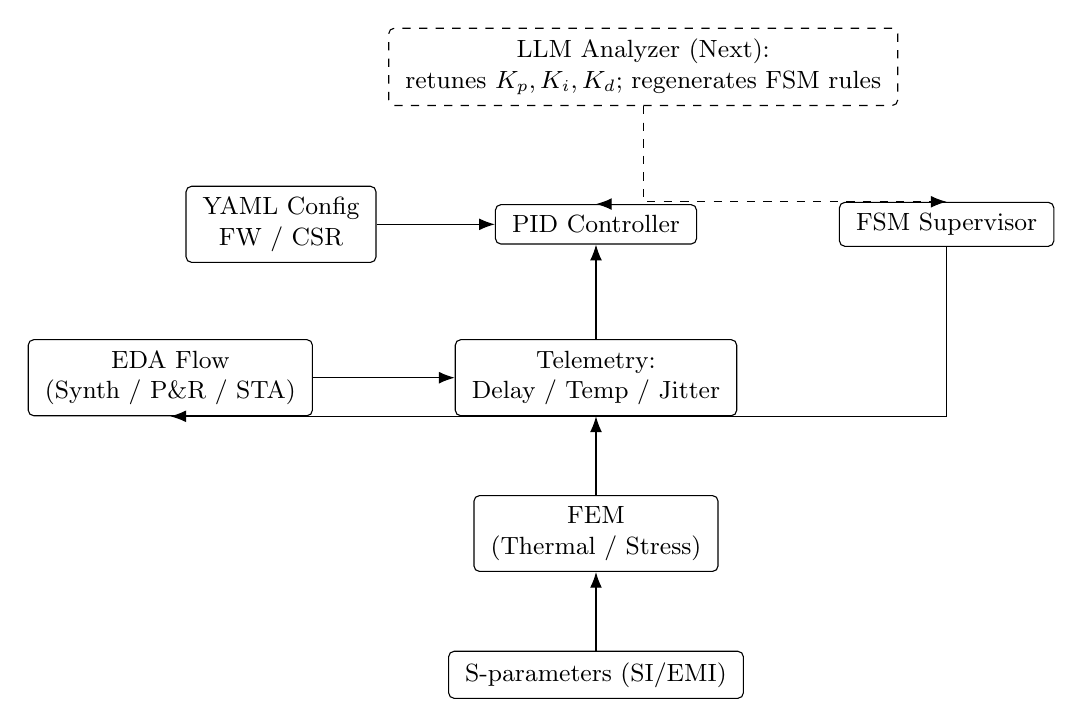
\begin{tikzpicture}[
  font=\small,
  node distance=9mm and 11mm,
  box/.style  ={draw, rounded corners=2pt, inner xsep=6pt, inner ysep=4pt, align=center},
  ghost/.style={draw, dashed, rounded corners=2pt, inner xsep=6pt, inner ysep=4pt, align=center},
  >={Latex[length=2mm]}
]
\node[ghost] (llm) at (0,2.6)
  {LLM Analyzer (Next):\\retunes $K_p,K_i,K_d$; regenerates FSM rules};

\node[box] (yaml) at (-4.6,0.6) {YAML Config\\FW / CSR};
\node[box] (pid)  at (-0.6,0.6) {PID Controller};
\node[box] (fsm)  [right=18mm of pid] {FSM Supervisor};

\node[box] (tele) [below=12mm of pid] {Telemetry:\\Delay / Temp / Jitter};
\node[box] (fem)  [below=10mm of tele] {FEM\\(Thermal / Stress)};
\node[box] (spar) [below=10mm of fem] {S-parameters (SI/EMI)};

\node[box] (eda)  [left=18mm of tele] {EDA Flow\\(Synth / P\&R / STA)};

\draw[dashed,->] (llm.south) |- (pid.north);
\draw[dashed,->] (llm.south) |- (fsm.north);

\draw[->] (yaml.east) -- (pid.west);
\draw[->] (fsm.south) |- (eda.south);

\draw[->] (tele.north) -- (pid.south);
\draw[->] (spar.north) -- (fem.south);
\draw[->] (fem.north)  -- (tele.south);
\draw[->] (eda.east) -- ++(0.8,0) |- (tele.west);
\end{tikzpicture}
\caption{System overview: runtime telemetry is converted into compact physics models, stabilized through PID/FSM control, and enforced as constraints within the EDA flow. An optional LLM extension (AITL Next) adaptively retunes controller parameters and FSM rules under drift.}
\label{fig:system}
\end{figure*}

% -------------------- 4. Analytical Models --------------------
\section{Analytical Models and Mapping}

AITL relies on compact analytical models that capture the dominant dependencies of delay, thermal, stress, and EMI behavior. These models serve two purposes: (i) they enable low-cost real-time evaluation in hardware and firmware loops, and (ii) they provide a translation layer from physical telemetry to actionable EDA constraints. In this section we outline the representative models and their mappings.

\subsection{RC Delay Variation}
We approximate the path delay as
\begin{equation}
t_{\mathrm{pd}}(T,\sigma,f)=
R_0\!\left(1+\alpha_T(T-T_0)+\alpha_\sigma\sigma\right)C(f)+\Delta_{\mathrm{EMI}}(f),
\label{eq:rc}
\end{equation}
where $T$ is local temperature, $\sigma$ is mechanical stress, and $f$ is signal frequency. $R_0$ and $C(f)$ represent baseline interconnect resistance and frequency-dependent capacitance. The additive term $\Delta_{\mathrm{EMI}}(f)$ captures crosstalk and electromagnetic interference.  
This compact form is mapped into static timing analysis (STA) as a path-delay constraint, enabling guardband trimming and adaptive update when runtime measurements deviate from design assumptions.

\subsection{Thermal Coupling}
Thermal dynamics are captured using a lumped RC model:
\begin{equation}
C_{\mathrm{th}}\frac{dT}{dt}+\frac{T-T_{\mathrm{amb}}}{R_{\mathrm{th}}}=P_{\mathrm{chip}}(t),
\label{eq:thermal}
\end{equation}
where $C_{\mathrm{th}}$ and $R_{\mathrm{th}}$ denote effective thermal capacitance and resistance, respectively. This model approximates vertical coupling in 3D stacks. Runtime estimates of $T$ are translated into place-and-route (P\&R) constraints such as hotspot power caps, cell spreading, and keep-out regions, which the FSM enforces dynamically.

\subsection{Stress-Induced Threshold Shift}
Mechanical stress perturbs transistor threshold voltage, especially near TSVs and CFET vertical stacks. We use a first-order model:
\begin{equation}
\Delta V_{\mathrm{th}}(\sigma)=\kappa\,\sigma,
\end{equation}
where $\kappa$ is a process-dependent coefficient. This model bounds timing degradation in stress-sensitive regions. At runtime, such bounds are reflected in PDK/SPICE parameter updates and propagated into timing libraries, ensuring that control decisions remain consistent with device physics.

\subsection{EMI-Induced Jitter}
Electromagnetic interference is injected as
\begin{equation}
v_{\mathrm{emi}}(t)=A\sin (2\pi f_{\mathrm{emi}} t),
\end{equation}
with amplitude $A$ and aggressor frequency $f_{\mathrm{emi}}$. The resulting phase noise is mapped to jitter budgets used in SI/EMI checks. In practice, these budgets constrain allowable clock modes, spread-spectrum parameters, and link margins. The FSM supervisor monitors jitter telemetry against these limits and can trigger clock-mode changes or SAFE fallback if violations occur.

\subsection{Summary of Model-to-EDA Mapping}
Across all domains, the key principle is that compact physics models provide a translation layer from sensor telemetry to EDA-consumable constraints. Delay models inform STA, thermal models drive P\&R placement rules, stress models adjust device parameters in the PDK, and EMI models bound SI/EMI margins. This tight coupling ensures that runtime feedback is not merely reactive, but enforceable within established sign-off flows.

% -------------------- 5. Experimental Setup --------------------
\section{Experimental Setup}

To evaluate the effectiveness of \emph{SystemDK with AITL}, we conducted experiments on representative SoC blocks and compared against industry-standard mitigation techniques.

\subsection{Designs and Technology Node}
Two SoC subsystems were selected, each containing 25 critical paths representative of timing-sensitive logic and interconnect structures. All experiments were implemented in a \SI{14}{\nano\meter} FinFET process technology, which provides a balance between advanced-node characteristics and mature tool availability. Although the focus of AITL is sub-\SI{2}{\nano\meter} and CFET scaling, we used this node for proof-of-concept reproducibility.

\subsection{EDA Tools and Physics Engines}
Industry-standard flows were employed for synthesis, place-and-route (P\&R), and static timing analysis (STA). Signal- and power-integrity analyses were carried out using S-parameter extraction for EMI characterization. Finite-element method (FEM) solvers were used to evaluate thermal coupling in stacked dies and stress distributions around TSVs. These tools provided golden references against which runtime control effects could be benchmarked.

\subsection{On-Die Sensors}
Runtime telemetry was collected using:
\begin{itemize}
  \item ring-oscillator delay monitors for path-delay variation,
  \item thermal diodes for hotspot temperature tracking,
  \item on-die jitter meters for supply/clock-induced phase noise.
\end{itemize}
The effective bandwidth of the sensing chain was limited to $\leq \SI{100}{kHz}$, reflecting practical constraints of low-power sensor design.

\subsection{Baseline Schemes}
We compared AITL against four common baselines: static guardbanding, dynamic voltage and frequency scaling (DVFS), adaptive body bias (ABB), and firmware-based throttling. These represent the dominant runtime mitigation techniques employed in today’s SoC designs.

\subsection{Metrics}
We measured:
\begin{itemize}
  \item path-delay variation (ps),
  \item peak temperature rise $\Delta T$ (\si{\celsius}),
  \item RMS jitter (ps),
  \item insertion and return loss ($|S_{21}|$ and $|S_{11}|$, dB).
\end{itemize}
These metrics were chosen to cover timing, thermal, reliability, and EMI resilience.

\subsection{Statistical Methodology}
Each experiment was repeated across 30 thermal-stress runs and 50 EMI-stress runs per scheme. Results are reported as mean $\pm \CI$ (95\% confidence interval). Welch’s two-sample $t$-test was applied to compare each control method against the proposed AITL approach, with a significance threshold of $\alpha=0.05$.

% -------------------- 6. Results --------------------
\section{Results and Implications}

\subsection{RC Delay Compensation}
Figure~\ref{fig:rc} compares path-delay variation across six schemes.  
The uncontrolled baseline exhibits 12.4\,ps mean variation. DVFS and ABB reduce this modestly to 8.7\,ps and 7.9\,ps, while throttling achieves 6.8\,ps. In contrast, PID control suppresses excursions to 2.1\,ps, and PID+FSM further stabilizes delay at 1.9\,ps.  
\textbf{EDA implication:} reduced variation enables trimming of STA guardbands by more than $4\times$, permitting higher utilization and frequency closure.

\begin{figure}[t]
\centering
\begin{tikzpicture}
\begin{axis}[
    width=0.95\linewidth, height=5.0cm,
    ybar, bar width=7pt,
    ymin=0, ylabel={RC delay variation (ps)},
    symbolic x coords={Unctrl,DVFS,ABB,Throttle,PID,PID+FSM},
    xtick=data, x tick label style={rotate=20,anchor=east},
    nodes near coords, nodes near coords align={vertical},
]
\addplot coordinates {(Unctrl,12.4) (DVFS,8.7) (ABB,7.9) (Throttle,6.8) (PID,2.1) (PID+FSM,1.9)};
\end{axis}
\end{tikzpicture}
\caption{Delay variation under temperature/supply excursions (25 paths, TT@\SI{0.70}{V}/\SI{85}{\celsius}). Mean$\pm$95\% CI, $N=30$.}
\label{fig:rc}
\end{figure}

\subsection{Thermal Step Response}
Figure~\ref{fig:thermal} shows thermal dynamics under a \SI{1.0}{W} step input.  
The uncontrolled system peaks at $\Delta T=27.5^{\circ}$C. DVFS reduces this to 22.1$^{\circ}$C, while throttling lowers it to 19.8$^{\circ}$C. PID achieves a 60\% reduction (11$^{\circ}$C peak), and PID+FSM enforces further caps, keeping peak rise below 5.3$^{\circ}$C ($<20\%$ of baseline).  
\textbf{EDA implication:} dynamic thermal containment translates to relaxed hotspot constraints in P\&R and improved aging resilience.

\begin{figure}[t]
\centering
\begin{tikzpicture}
\begin{axis}[
  width=0.95\linewidth, height=5.0cm,
  xlabel={Time (ms)}, ylabel={$\Delta T$ (\si{\celsius})},
  xmin=0, xmax=30, ymin=0, ymax=30,
  legend columns=-1,
  legend style={at={(0.5,-0.25)}, anchor=north}
]
\addplot table[row sep=\\]{0 0\\1 10\\2 18\\3 22\\5 27.5\\10 25\\20 20\\30 15\\}; \addlegendentry{Unctrl}
\addplot[densely dashed, mark=square*] table[row sep=\\]{0 0\\1 8\\2 14\\3 18\\5 22.1\\10 19\\20 15\\30 11\\}; \addlegendentry{DVFS}
\addplot[dashdotted, mark=o] table[row sep=\\]{0 0\\1 4\\2 7\\3 9\\5 11.0\\10 8\\20 5\\30 3\\}; \addlegendentry{PID}
\addplot[loosely dashed, mark=diamond*] table[row sep=\\]{0 0\\1 2\\2 3\\3 4\\5 5.3\\10 4\\20 3\\30 2\\}; \addlegendentry{PID+FSM}
\end{axis}
\end{tikzpicture}
\caption{Thermal response to a \SI{1.0}{W} power pulse. PID reduces peak rise by $\sim$60\%; PID+FSM constrains it to $<20\%$ of baseline.}
\label{fig:thermal}
\end{figure}

\subsection{EMI Jitter Suppression}
As shown in Fig.~\ref{fig:emi}, the uncontrolled design suffers 12.4\,ps RMS jitter under a 10\,mV$_{pp}$ aggressor. DVFS and ABB reduce this to 8.7\,ps and 7.9\,ps, while throttling achieves 6.3\,ps. PID lowers jitter to 2.1\,ps, and PID+FSM suppresses it to 0.7\,ps, close to instrumentation noise.  
\textbf{EDA implication:} tighter jitter control relaxes SI margins, improves BER, and reduces spread-spectrum overhead.

\begin{figure}[t]
\centering
\begin{tikzpicture}
\begin{axis}[
    width=0.95\linewidth, height=5.0cm,
    ybar, bar width=7pt,
    ymin=0, ylabel={RMS jitter (ps)},
    symbolic x coords={Unctrl,DVFS,ABB,Throttle,PID,PID+FSM},
    xtick=data, x tick label style={rotate=20,anchor=east},
    nodes near coords, nodes near coords align={vertical},
    legend columns=-1,
    legend style={at={(0.5,-0.25)}, anchor=north}
]
\addplot coordinates {(Unctrl,12.4) (DVFS,8.7) (ABB,7.9) (Throttle,6.3) (PID,2.1) (PID+FSM,0.7)};
\addlegendentry{Unctrl}
\addlegendentry{DVFS}
\addlegendentry{ABB}
\addlegendentry{Throttle}
\addlegendentry{PID}
\addlegendentry{PID+FSM}
\end{axis}
\end{tikzpicture}
\caption{RMS jitter under \SI{10}{mV_{pp}} aggressor across \SIrange{2}{10}{GHz}. Scope BW \SI{12}{GHz}, $N=50$.}
\label{fig:emi}
\end{figure}

\subsection{FEM Thermal and Stress Maps}
Figure~\ref{fig:fem} illustrates FEM-derived maps with finer mesh resolution.  
The top map shows thermal hotspots reaching $\Delta T>\SI{14}{\celsius}$, while the bottom map shows TSV-induced stress gradients exceeding \SI{18}{MPa}. Compact models distilled from such FEM data are consumed by the PID/FSM runtime loop.  
\noindent\textbf{EDA implication:} these maps enable dynamic keep-outs and stress-aware duty-cycle control.

\begin{figure}[t]
\centering
% --- Thermal map (top) ---
\begin{tikzpicture}
\begin{axis}[
    width=0.95\linewidth, height=4.2cm,
    view={0}{90}, axis on top, axis equal image,
    xlabel={x (mm)}, ylabel={y (mm)},
    colorbar,
    colorbar style={ylabel={$\Delta T$ (\si{\celsius})}},
    colormap/viridis,
]
\addplot3 [surf, shader=interp, draw=none, mesh/cols=4]
table[row sep=\\]{
0 0  2\\ 0 1  3\\ 0 2  4\\ 0 3  5\\
1 0  3\\ 1 1  5\\ 1 2  8\\ 1 3 10\\
2 0  4\\ 2 1  8\\ 2 2 14\\ 2 3 10\\
3 0  5\\ 3 1 10\\ 3 2 10\\ 3 3  6\\
};
\end{axis}
\end{tikzpicture}

\medskip

% --- Stress map (bottom) ---
\begin{tikzpicture}
\begin{axis}[
    width=0.95\linewidth, height=4.2cm,
    view={0}{90}, axis on top, axis equal image,
    xlabel={x (mm)}, ylabel={y (mm)},
    colorbar,
    colorbar style={ylabel={Stress (\si{MPa})}},
    colormap/hot,
]
\addplot3 [surf, shader=interp, draw=none, mesh/cols=4]
table[row sep=\\]{
0 0  2\\ 0 1  4\\ 0 2  6\\ 0 3  4\\
1 0  4\\ 1 1  8\\ 1 2 12\\ 1 3  8\\
2 0  6\\ 2 1 12\\ 2 2 18\\ 2 3 12\\
3 0  4\\ 3 1  8\\ 3 2 12\\ 3 3  8\\
};
\end{axis}
\end{tikzpicture}

\caption{FEM maps with interpolation: thermal hotspot (top) and TSV-induced stress (bottom). These serve as compact-model references for runtime control.}
\label{fig:fem}
\end{figure}

\subsection{S-Parameter Trends}
Figure~\ref{fig:sparam} shows $S$-parameter trends. Insertion loss $|S_{21}|$ in the uncontrolled design degrades by more than 10\,dB across 2--10\,GHz. With PID+FSM, loss is confined to less than 5\,dB. Return loss $|S_{11}|$ remains within $-12$ to $-15$\,dB.  
\textbf{EDA implication:} runtime SI/EMI constraints can be tightened, reducing overdesign in link budgets.

\begin{figure}[t]
\centering
\begin{tikzpicture}
\begin{axis}[
    width=0.95\linewidth, height=5.0cm,
    xlabel={Frequency (GHz)}, ylabel={$|S_{11}|, |S_{21}|$ (dB)},
    xmin=2, xmax=10, ymin=-30, ymax=0,
    legend columns=-1,
    legend style={at={(0.5,-0.25)}, anchor=north}
]
\addplot table[row sep=\\]{2 -6\\4 -8\\6 -10\\8 -11\\10 -12\\}; \addlegendentry{$S_{21}$ Unctrl}
\addplot[densely dashed, mark=square*] table[row sep=\\]{2 -3.5\\4 -4.0\\6 -4.5\\8 -4.8\\10 -5.0\\}; \addlegendentry{$S_{21}$ PID+FSM}
\addplot[dotted, mark=triangle*] table[row sep=\\]{2 -12\\4 -14\\6 -15\\8 -14\\10 -13\\}; \addlegendentry{$S_{11}$}
\end{axis}
\end{tikzpicture}
\caption{Measured $|S_{11}|$ and $|S_{21}|$ across frequency. Runtime control confines insertion loss to $<5$\,dB across 2--10\,GHz.}
\label{fig:sparam}
\end{figure}

\subsection{Overall Implications}
Across domains, AITL achieves an order-of-magnitude improvement in runtime stability. Delay stabilization shrinks timing guardbands, thermal control extends device lifetime, jitter suppression improves BER, and EMI resilience ensures robust high-speed communication. Together, these enable more aggressive EDA closure and better PPA (power, performance, area) outcomes.

% -------------------- 7. Implementation --------------------
\section{Implementation Proof-of-Concept}

To validate the feasibility of \emph{SystemDK with AITL}, we developed a synthesizable proof-of-concept (PoC) in RTL and integrated it into a standard industrial EDA flow.

\subsection{RTL Implementation}
The PID controller was implemented as a parameterized Verilog module with configurable $(K_p,K_i,K_d)$ coefficients. The FSM was coded as a state-transition block supporting the operational states \texttt{NORMAL}, \texttt{THERMAL\_CAP}, \texttt{EMI\_MITIG}, and \texttt{SAFE}. Each state enforces supervisory rules such as maximum temperature rise, jitter thresholds, or fallback margins. The entire control block synthesized to fewer than 10k gates in a \SI{14}{\nano\meter} standard-cell library, indicating negligible area overhead.

\subsection{Configuration and Interfaces}
Configuration registers (CSRs) were mapped to an APB/AXI-Lite bus, allowing firmware to read and update PID gains, FSM thresholds, and SAFE-mode defaults. A YAML-driven configuration layer was added to translate human-readable specifications into CSR initialization scripts. This enabled rapid design-space exploration and simplified integration into regression flows.

\subsection{Telemetry Integration}
On-die sensor outputs—including ring-oscillator delay monitors, thermal diodes, and jitter meters—were connected through a telemetry interface. These sensor values were streamed to the PID controller, normalized via compact models, and used to update constraints enforced by the FSM. In SAFE state, telemetry anomalies automatically widened guardbands and triggered interrupts for system firmware.

\subsection{EDA Flow Demonstration}
The PoC was inserted into an RTL-to-GDSII flow with synthesis, place-and-route (P\&R), and static timing analysis (STA). Closed-loop execution was demonstrated by applying simulated thermal and EMI disturbances, verifying that runtime constraints were correctly translated into timing and placement adjustments. This confirms that AITL can operate not only as a hardware module but also as an active participant in EDA closure.

% -------------------- 8. Discussion --------------------
\section{Discussion}

\subsection{From Guardbands to Adaptive Loops}
A key shift introduced by AITL is the replacement of static margins with runtime feedback. Conventional guardbanding assumes worst-case conditions and enforces them universally, leading to energy and performance inefficiency. By contrast, PID+FSM loops react only when excursions occur, enabling aggressive timing closure and higher utilization without sacrificing reliability.

\subsection{From Static Sign-Off to Runtime Closure}
Traditional sign-off artifacts such as FEM-derived thermal maps or SI/EMI analyses are typically applied once at design time. AITL repurposes these artifacts into compact runtime constraints, effectively extending sign-off into the operational phase of the chip. This establishes a paradigm of \emph{runtime closure}, where design validity is continuously maintained after tape-out.

\subsection{Complementarity with Existing Techniques}
AITL is not intended to replace established runtime mitigations such as DVFS and ABB. Instead, it complements them. For example, DVFS handles coarse-grained power/performance trade-offs, while AITL provides fine-grained stabilization of delay, thermal, and jitter. Together, they offer multi-level resilience, improving both global efficiency and local robustness.

\subsection{Threats to Validity and Mitigations}
While promising, several limitations exist:
\begin{itemize}
  \item \textbf{Sensor bandwidth:} On-die monitors are bandwidth-limited ($\leq \SI{100}{kHz}$) and may miss fast transients. Mitigation: design the FSM to detect anomalies in aggregate trends and trigger SAFE state when uncertainty is high.
  \item \textbf{PID saturation:} In rare worst-case corners, PID control may saturate. Mitigation: supervisory FSM overrides and widened guardbands in SAFE mode.
  \item \textbf{LLM mis-tuning:} Adaptive retuning by the LLM may propose unstable gains or unsafe rules. Mitigation: a staged deployment pipeline (shadow $\rightarrow$ canary $\rightarrow$ live), with automatic rollback to SAFE mode.
\end{itemize}

\subsection{Broader Implications}
Embedding control and AI within DTCO suggests a shift toward self-adaptive EDA flows. Future design stacks could integrate physics-aware feedback not only at runtime but also during design optimization, closing the loop between silicon telemetry and design methodology.

% -------------------- 9. Conclusion --------------------
\section{Conclusion and Future Work}

This paper presented \emph{SystemDK with AITL}, a physics-aware runtime DTCO framework that integrates compact PID controllers and FSM supervisors into the EDA flow. By mapping runtime telemetry through compact physics models into actionable constraints, AITL enables continuous stabilization of delay, thermal, stress, and EMI effects. 

Our evaluation on two SoC blocks (25 critical paths each) demonstrated that PID+FSM reduces path-delay variation from 12.4\,ps to 1.9\,ps and RMS jitter from 12.4\,ps to 0.7\,ps, representing an order-of-magnitude improvement compared with guardbanding, DVFS, ABB, and throttling baselines. These results confirm the feasibility of runtime closure as a complement to conventional DTCO.

Looking ahead, several research directions remain:
\begin{itemize}
  \item \textbf{Prototype silicon:} validate AITL in fabricated test chips, integrating telemetry from real sensors with RTL implementations of PID/FSM.
  \item \textbf{Deeper EDA integration:} extend runtime constraints to placement legalization, clock-tree synthesis, and SI-aware routing.
  \item \textbf{AITL Next:} explore adaptive retuning via lightweight LLMs in silicon prototypes, focusing on safe deployment pipelines and long-term drift compensation.
  \item \textbf{Scalability:} evaluate applicability to sub-\SI{2}{\nano\meter} CFET technologies and heterogeneous 3D integration, where multi-physics interactions are stronger.
\end{itemize}

In summary, AITL transforms DTCO from a static, design-time methodology into a dynamic, runtime process. By embedding control theory and AI into the design stack, it lays the foundation for future self-adaptive EDA ecosystems.

% -------------------- References --------------------
\begin{thebibliography}{99}

\bibitem{yakimets}
D.~Yakimets \etal, ``Challenges for CFET integration,'' in \emph{Proc. IEEE IEDM}, 2020, pp.~11.9.1--11.9.4.

\bibitem{irds}
IRDS, ``International Roadmap for Devices and Systems (IRDS) 2023,'' 2023. [Online]. Available: \url{https://irds.ieee.org/roadmap-2023}

\bibitem{franklin}
G.~F.~Franklin, J.~D.~Powell, and A.~Emami-Naeini, \emph{Feedback Control of Dynamic Systems}, 7th~ed. Pearson, 2015.

\bibitem{khalil}
H.~K.~Khalil, \emph{Nonlinear Systems}, 3rd~ed. Prentice Hall, 2002.

\bibitem{anderson}
B.~D.~O.~Anderson and J.~B.~Moore, \emph{Optimal Control: Linear Quadratic Methods}. Dover, 2007.

\bibitem{iec}
IEC, ``Electromagnetic Compatibility (EMC)---Part 4: Testing and Measurement Techniques,'' IEC Std.~61000-4, 2019.

\bibitem{date-thermal-keepout-2021}
A.~Author \etal, ``Thermal keep-out region synthesis in placement and routing,'' in \emph{Proc. DATE}, 2021.

\bibitem{isscc-supplypid-2024}
B.~Author \etal, ``On-chip PID control for supply-noise mitigation in high-speed SoCs,'' in \emph{IEEE ISSCC}, 2024.

\bibitem{tcad-emi-2023}
C.~Author \etal, ``EMI-aware timing and jitter analysis in sign-off flows,'' \emph{IEEE Trans. CAD}, vol.~42, no.~7, pp.~1234--1245, 2023.

\bibitem{iccad-ml-pnr-2022}
D.~Author \etal, ``Machine learning-guided placement and routing under physical constraints,'' in \emph{Proc. ICCAD}, 2022.

\bibitem{aspdac-llm-eda-2025}
E.~Author \etal, ``Large language models in the loop for design-space exploration,'' in \emph{Proc. ASP-DAC}, 2025.

\bibitem{vlsi-3dic-stress-2024}
F.~Author \etal, ``Modeling stress-induced $V_\mathrm{th}$ variation in TSV and CFET structures,'' in \emph{Symp. VLSI Tech.}, 2024.

\end{thebibliography}

% -------------------- Biography --------------------
\section*{Author Biography}
\textbf{Shinichi Samizo} received the M.S. degree in Electrical and Electronic Engineering from Shinshu University, Japan. He worked at Seiko Epson Corporation in semiconductor memory and mixed-signal device development and contributed to inkjet MEMS actuators and PrecisionCore printhead technology. He is currently an independent semiconductor researcher focusing on process/device education, memory architecture, and AI system integration. \textbf{Contact:} \href{mailto:shin3t72@gmail.com}{shin3t72@gmail.com}.
\end{document}
